\subsection{The class associated with an exact sequence}

PROPOSITION 1. --- Let (C, d) and (C', d') be two complexes of left A-modules and n, p, q three integers such that \(p \geqslant q\) . For \(p \geqslant i \geqslant q - 1\) , let \(f_i: C_i \to C_{i+n+1}'\) be a homomorphism of A-modules such that \(f_p \circ d = 0\) , \(f_i \circ d = d' \circ f_{i+1}\) for \(p > i \geqslant q - 1\) , and \(d' \circ f_{q-1} = 0\) (see fig.~2).

\pandocbounded{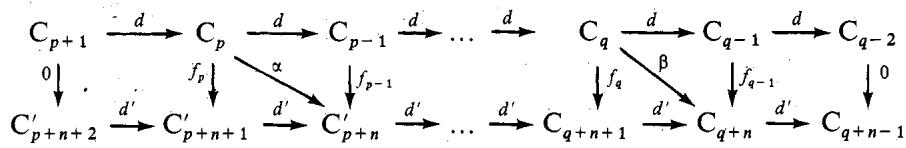
\includegraphics[keepaspectratio]{images/part001_b19b44e0.jpg}}\\
FIG. 2.

Set \(\alpha = f_{p-1} \circ d = d' \circ f_p\) , \(\beta = f_{q-1} \circ d = d' \circ f_q\) , and let \(a\) (resp. \(b\) ) be the graded A-homomorphism of degree \(n\) from C to C' whose only nonzero bihomogeneous component is \(\alpha\) (resp. \(\beta\) ). Then one has \(a \in Z_n(\text{Homgr}_A(C, C'))\) , \(b \in Z_n(\text{Homgr}_A(C, C'))\) and \(a - (-1)^{(n+1)(p-q)} b \in B_n(\text{Homgr}_A(C, C'))\) .

One has \(d' \circ \alpha = d' \circ d' \circ f_p = 0\) , \(\alpha \circ d = f_{p-1} \circ d \circ d = 0\) , hence

\[
a \in Z _ {n} \left(\operatorname{Homgr} _ {\mathrm{A}} \left(\mathrm{C}, \mathrm{C} ^ {\prime}\right)\right);
\]

likewise \(b \in Z_n(\text{Homgr}_A(C, C'))\) . Set \(\varepsilon = (-1)^{n+1}\) . One has, in the complex \(\text{Homgr}_A(C, C')\) the relations

\[
\mathrm{D} f _ {p - 1} = d ^ {\prime} \circ f _ {p - 1} - \varepsilon f _ {p - 1} \circ d = f _ {p - 2} \circ d - \varepsilon \alpha
\]

\[
\mathrm{D} f _ {i} = d ^ {\prime} \circ f _ {i} - \varepsilon f _ {i} \circ d = f _ {i - 1} \circ d - \varepsilon f _ {i} \circ d (p - 1 > i > q)
\]

\[
\mathrm{D} f _ {q} = d ^ {\prime} \circ f _ {q} - \varepsilon f _ {q} \circ d = \beta - \varepsilon f _ {q} \circ d,
\]

hence

\[
\sum_ {i = 1} ^ {p - q} \varepsilon^ {i} D f _ {p - i} = \varepsilon^ {p - q} \beta - \alpha ,
\]

which proves the lemma.

Consider two left A-modules M and N and an exact sequence of A-modules

\[
0 \rightarrow \mathrm{N} \rightarrow \mathrm{R} _ {n} \rightarrow \mathrm{R} _ {n - 1} \rightarrow \dots \rightarrow \mathrm{R} _ {1} \rightarrow \mathrm{M} \rightarrow 0.\tag{4}
\]

By props. 3 and 3 bis of X, p.~49, there exists a commutative diagram:

\begin{enumerate}
\def\labelenumi{(\arabic{enumi})}
\setcounter{enumi}{4}
\tightlist
\item
\end{enumerate}

\pandocbounded{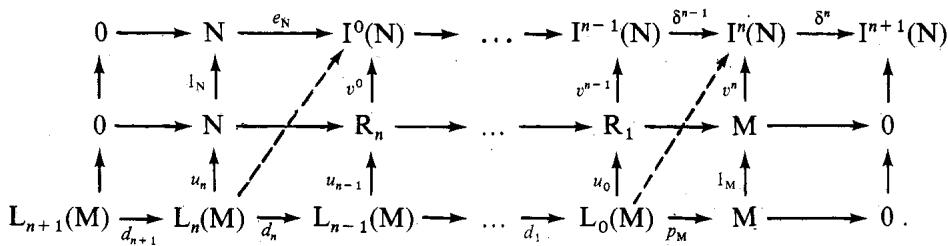
\includegraphics[keepaspectratio]{images/part001_efe78803.jpg}}

Consider the two elements \(b\) and \(a\) of \(\mathrm{Homgr}_{\mathbf{A}}(\mathrm{L}(\mathbf{M}),\mathrm{I}(\mathbf{N}))\) whose only nonzero bihomogeneous components are

\[
b ^ {n} = e _ {\mathrm{N}} \circ u _ {n}: \mathrm{L} _ {n} (\mathrm{M}) \rightarrow \mathrm{I} ^ {0} (\mathrm{N}) \quad \text { and } \quad a ^ {n} = v ^ {n} \circ p _ {\mathrm{M}}: \mathrm{L} _ {0} (\mathrm{M}) \rightarrow \mathrm{I} ^ {n} (\mathrm{N})
\]

respectively.

PROPOSITION 2. --- One has \(a\) , \(b \in Z^n(\text{Homgr}_A (\text{L(M)}, \text{l(N)})\) ). Moreover, the classes \(\overline{a}\) and \(\overline{b}\) of \(a\) and \(b\) in \(\text{H}^n(\text{Homgr}_A (\text{L(M)}, \text{l(N)})) = \text{Ext}_A^n (\text{M}, \text{N})\) depend only on the exact sequence (4) and are equal.

By prop. 1, applied to the two extreme rows of (5) and to the composed vertical arrows, with \(p = n\) , \(q = 0\) , we have \(a\) , \(b \in \mathbf{Z}^{n}(\mathrm{Homgr}_{\mathrm{A}}(\mathrm{l(M)}, \mathrm{L(N)}))\) and

\[
a - b = a - (- 1) ^ {(n + 1) n} b \in \mathrm{B} ^ {n} (\operatorname{Homgr} _ {\mathrm{A}} (\mathrm{L} (\mathrm{M}), \mathrm{I} (\mathrm{N}))).
\]

Since \(a\) (resp. \(b\) ) is independent of the choice of \(u\) (resp. \(v\) ), the element \(\overline{a} = \overline{b}\) of \(\mathrm{Ext}_{\mathbf{A}}^{n}\) (M, N) is independent of the choice of morphisms \(u\) and \(v\) , whence the proposition.

DEFINITION 1. --- The element \(\theta\) of \(\operatorname{Ext}_{\mathbf{A}}^{n}(\mathbf{M}, \mathbf{N})\) defined by \(\theta = (-1)^{n(n+1)/2} \overline{a} = (-1)^{n(n+1)/2} \overline{b}\) is called the class associated with the exact sequence (4) .

Remarks. --- 1) Let (P, p) be a projective resolution of M. By X, p.~49, prop. 3, there exists a commutative diagram

\[
\begin{array}{c} 0 \longrightarrow \mathrm{N} \longrightarrow \mathrm{R} _ {n} \longrightarrow \dots \longrightarrow \mathrm{R} _ {1} \longrightarrow \mathrm{M} \longrightarrow 0 \\ \tilde {u} _ {n} \uparrow \quad \tilde {u} _ {n - 1} \uparrow \quad \tilde {u} _ {0} \uparrow \quad \uparrow_ {\mathrm{M}} \\ \mathrm{P} _ {n} \longrightarrow \mathrm{P} _ {n - 1} \longrightarrow \dots \longrightarrow \mathrm{P} _ {0} \xrightarrow {p} \mathrm{M} \longrightarrow 0. \end{array}
\]

With the notations of § 6, θ is the image under φ(P, N) of the homotopy class of the morphism P → N defined by \((-1)^{n(n+1)/2} \tilde{u}_{n}\) . Similarly, if \((e, E)\) is an injective resolution of N, there exists a commutative diagram

\[
\begin{array}{c} 0 \longrightarrow \mathrm{N} \longrightarrow \mathrm{E} ^ {0} \longrightarrow \dots \longrightarrow \mathrm{E} ^ {n - 1} \longrightarrow \mathrm{E} ^ {n} \\ 1 _ {\mathrm{N}} \uparrow \quad \tilde {v} ^ {0} \uparrow \quad \quad \quad \quad \quad \quad \quad \quad \quad \quad \quad \quad \quad \quad \quad \quad \quad \quad \quad \quad \quad \quad \quad \quad 0 \longrightarrow \mathrm{N} \longrightarrow \mathrm{R} _ {n} \longrightarrow \dots \longrightarrow \mathrm{R} _ {1} \longrightarrow \mathrm{M} \longrightarrow 0. \end{array}
\]

and \(\theta\) is the image under \(\varphi(\mathbf{M},\mathbf{E})\) of the homotopy class of the morphism \(\mathbf{M}\to\mathbf{E}\) defined by \((-1)^{n(n+1)/2}v^{n}\) . This follows from the construction of \(\theta\) and definitions of \(\varphi(\mathbf{P},\mathbf{N})\) and \(\varphi(\mathbf{M},\mathbf{E})\) .

\begin{enumerate}
\def\labelenumi{\arabic{enumi})}
\setcounter{enumi}{1}
\tightlist
\item
  When \(n = 0\) , the exact sequence (4) is written \(0 \to \mathbf{N} \xrightarrow{f} \mathbf{M} \to 0\) , and the associated class is \(f^{-1} \in \operatorname{Hom}_{\mathbf{A}}(\mathbf{M}, \mathbf{N}) = \operatorname{Ext}_{\mathbf{A}}^{0}(\mathbf{M}, \mathbf{N})\) .
\end{enumerate}

